\documentclass[conference]{IEEEtran}
\usepackage[utf8]{inputenc}
\usepackage[spanish]{babel}
\usepackage{multirow}
\usepackage{amsmath}
\usepackage{float}
\usepackage{fancyhdr}

%------------------- Encabezado y Pie de pág -------------------
\pagestyle{fancy}
\fancyhf{}
\lhead{Electrónica de Potencia}
\rhead{Página \thepage}
%----------------------------------------------------


\ifCLASSINFOpdf
\usepackage[pdftex]{graphicx}


\else
\fi
\hyphenation{op-tical net-works semi-conduc-tor}

\begin{document}
\title{Robustez y desempeño de los MOSFET's y los IGBT's durante su operación en cortocircuito.}
\author{
		\begin{tabular}{c}
			\textbf{Navarro, Facundo Emilio - @63809@electronica.frc.utn.edu.ar} \\ 
			Estudiante de Ingeniería Electrónica - Universidad Tecnológica Nacional - Facultad Regional Córdoba.\\
	\textit{Paper número 9541-30/19}
		\end{tabular}
		}
\maketitle

\begin{abstract}
Tanto los transistores MOSFET's (Metal Oxide Semiconductor Field Effect Transistor) como los IGBT's (Insulated Gate Bipolar Transistor) son dispositivos de potencia controlados por tensión que se utilizan principalmente en conmutación. El primero de ellos fue desarrollado como consecuencia de la búsqueda de una alternativa a las limitaciones de los BJT; mientras que los IGBT's combinan algunas de las mejores propiedades de los MOSFET's y de los BJT, ya que ellos son parte de su estructura interna. Este trabajo plantea un análisis del comportamiento de ambos dispositivos bajo la condición de cortocircuito, la cual es muy utilizada en aplicaciones de conmutación, sin que ello pueda significarle un perjuicio.\\

\textit{Abstract}--- As much the MOSFET's transistors (Metal Oxide Semiconductor Field Effect Transistor) like the IGBT's (Insulated Bipolar Gate Transistor) are devices of power controlled by tension that are used mainly in commutation.  First of them it was developed as a result of the search of an alternative to the limitations of the BJT;  whereas the IGBT's combines some of the best properties of the MOSFET's and the BJT, since they are part of their internal structure.  This work raises an analysis of the behavior of both devices under the condition of short circuit, which is very used in applications of commutation, without this can mean a damage to them.
\end{abstract} 

\IEEEpeerreviewmaketitle

\section*{Nomenclatura}
\begin{table}[H]
\centering
\begin{tabular}{lccl}
$DC$    & & & Corriente continua        \\
$SOA$  	& & & Área de operación segura. \\
$I_D$ 	& & & Corriente de drenador.   	\\
$I_C$ 	& & & Corriente de colector.  	\\
$Q_{rr}$& & & Carga de recuperación inversa del diodo del cuerpo.
\end{tabular}
\end{table}

\section{Introducción}
\label{sec:intro}

El rendimiento de los dispositivos semiconductores de potencia mejora continuamente en respuesta a las demandas cada vez mayores de aplicaciones más eficientes energéticamente hablando. La evolución de los dispositivos de semiconductores de potencia siempre se han centrado en aumentar las potencias nominales, mientras que al mismo tiempo mejora el rendimiento del dispositivo en términos de eficiencia, mayor densidad de potencia, mayor robustez y confiabilidad en condiciones normales y anormales

Las propiedades que llevan al MOSFET a ser la elección predilecta a la hora de realizar diseños de potencia son su gran capacidad de conmutar en altas velocidades, el fácil manejo, la capacidad de avalancha y el gran área de operación segura (SOA). Estas ventajas son parcialmente malogradas por sus características de conducción. Además, a medida que la tensión máxima de ruptura aumenta se incrementan las pérdidas en el dispositivo. Los IGBT además de compartir algunas de las propiedades de los MOSFET, poseen características de conducción superiores. Generalmente la velocidad de conmutación del IGBT es inferior a la del MOSFET, pero en los últimos años se han desarrollado nuevas líneas de IGBT que poseen características de conmutación muy cercanas a los MOSFET sin tener que sacrificar las características de mejor conducción. 

Las industrias todavía están luchando con modos de falla que son impredecibles, también conocidos por la curva de la bañera \cite{bath} como fallas aleatorias. Las fallas aleatorias o catastróficas son las que no se pueden predecir porque no muestran ninguna evidencia antes de la falla, solo después del análisis posterior a la falla y la comprensión de la causa, es posible rediseñar el componente para mitigar el problema.

\subsubsection{Cortocircuitos}
En los circuitos electrónicos de potencia, puede producirse un cortocircuito de muchas maneras diferentes; el los más comunes son el tipo 1 y el tipo 2 (Figura \ref{fig:sc1}).
\begin{figure}[H]
	\centering
	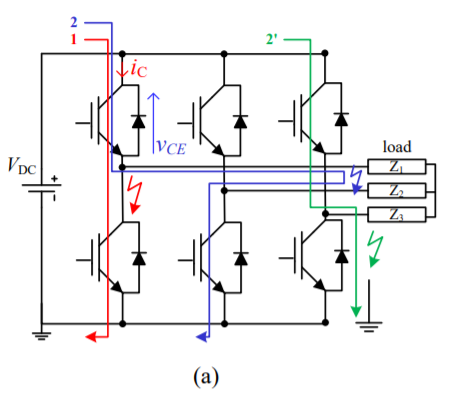
\includegraphics[width=\columnwidth]{imagenes/sc1}
	\caption{Caminos de cortocircuito en un convertidor de fuente de voltaje trifásico. \cite{sc}}
	\label{fig:sc1}
\end{figure}

La Fig. \ref{fig:sc1} muestra un convertidor trifásico tradicional comúnmente encontrado en aplicaciones de motores. 

El tipo 1 de cortocircuito es un cortocircuito que ya existe cuando el dispositivo bajo prueba está encendido (trayectoria 1 en la Fig. \ref{fig:sc1}). Esta situación ocurre cuando los IGBT superiores e inferiores están en conducción.
 Por otro lado, el cortocircuito tipo 2 es un cortocircuito que tiene lugar cuando el IGBT está conduciendo. En este caso, la falla se puede observar desde la rama a fase (ver el camino 2 en la Fig. \ref{fig:sc1}) y desde esa rama del puente a tierra (ver la ruta 2 en la Fig. \ref{fig:sc1}). Durante el evento de cortocircuito, el IGBT puede resistir la sobrecarga y ser apagado con éxito por el conductor del gate, o por el contrario, podría conducir a una falla catastrófica.

 Las fallas de cortocircuito se pueden clasificar en cuatro, dependiendo del momento en que se produce el fallo, como se muestra en la Fig. \ref{fig:sc2}. 
 
 \begin{figure}[H]
	\centering
	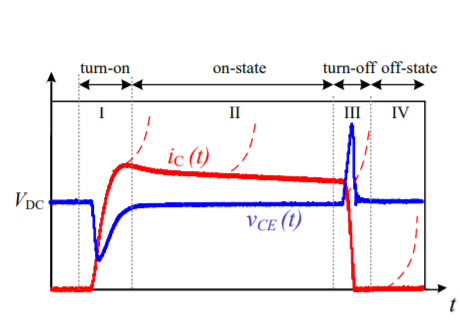
\includegraphics[width=\columnwidth]{imagenes/sc2}
	\caption{Tipos de fallas durante un cortocircuito. \cite{sc}}
	\label{fig:sc2}
\end{figure}
 
 \begin{itemize}
 \item  El primer modo de falla ocurre durante el transitorio de encendido, por ejemplo, una falla del dispositivo en sí debido a algún tipo de inestabilidad.
 \item El segundo modo de falla ocurre durante el estado de encendido, por ejemplo si la energía disipada es mayor que un valor crítico.
 \item El tercero el modo de falla ocurre durante el apagado transitorio, por una sobretensión de gran voltaje.
 \item El cuarto modo de falla ocurre durante el estado apagado, generalmente relacionado con una fuga aumento actual que causa fallas térmicas fuera de control.
 \end{itemize}
 


\section{MOSFET e IGBT en cortocircuto}
Hoy en día, una amplia gama de aplicaciones críticas para la energía pueden beneficiarse de la baja figura de mérito de los "trench"  MOSFET ($R_{DS_{(on)}} \cdot  Q_{g}$) debido a los altos voltajes de bloqueo de los MOSFET.

Sin embargo, la $R_{DS_{(on)}}$ y $Q$ no son los únicos parámetros que deben tenerse en cuenta al elegir MOSFET adecuados para una aplicación. Un aspecto a menudo descuidado pero esencial cuando se trata de la selección MOSFET para aplicaciones de conmutación dura es la conmutación dura del diodo del cuerpo. La resistencia insuficiente del diodo del cuerpo puede conducir a una falla del sistema y el problema se vuelve cada vez más grave a medida que aumenta el voltaje de ruptura.

En los convertidores de conmutación, los diodos del cuerpo son instrumentos comunes que se utilizan para proporcionar la capacidad de paso libre sin costo adicional de componentes. Es una ventaja en este caso ya que no se requiere de un diodo externo. Sin embargo, el comportamiento de recuperación en inversa si es descuidado menudo podría causar anomalías en el dispositivo y provocar fallas en el sistema. Para seleccionar correctamente los tipos de MOSFET de alto voltaje, se vuelve cada vez más importante considerar el evento de conmutación dura, y un sistema confiable requiere una selección cuidadosa de los MOSFET con diodos de cuerpo robustos para cumplir con los requisitos de la aplicación.

Durante la transición de apagado de conmutación dura, el diodo se polariza inicialmente hacia adelante y transporta una corriente directa positiva. Tan pronto como se inicia el proceso de apagado, la corriente baja a una pendiente constante ($\frac{d_i}{d_t}$) a cero, luego invierte la dirección. La corriente negativa, también conocida como corriente de recuperación inversa ($I_{rr}$), finalmente alcanza el pico negativo ($I_{{rr}_{m}}$) y luego vuelve a cero. El proceso de recuperación inversa se completa en este momento, y el diodo del cuerpo vuelve a su estado de bloqueo.


En los MOSFET's los tiempos de conmutación son determinados principalmente por la acción conjunta de sus capacitancias internas e inductancias y la resistencia interna de la fuente de tensión del control de compuerta; el circuito que se utiliza para medir los tiempos de conmutación de un MOSFET puede verse en la Fig. \ref{fig:circuit_mosfet}, y los tiempos de conmutación de un MOSFET IRF150 se encuentran representados en las Figuras \ref{fig:vds_mosfet}, \ref{fig:vgs_mosfet} y \ref{fig:vds_vgs_mosfet}. 


\begin{figure}[H]
	\centering
	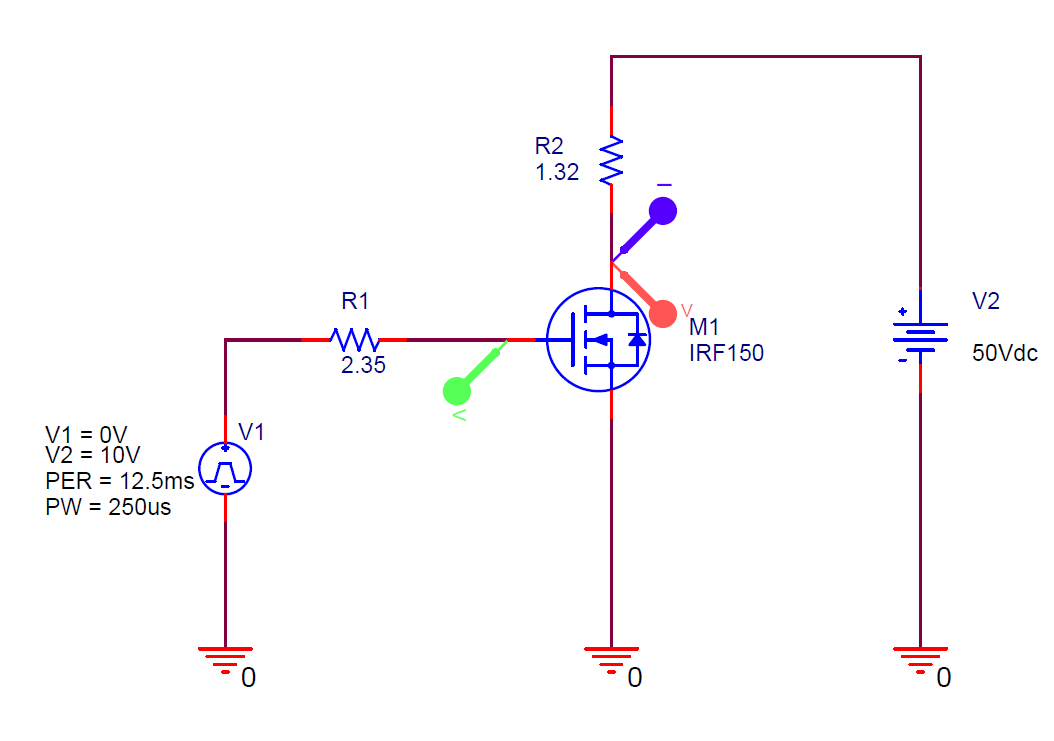
\includegraphics[width=\columnwidth]{imagenes/circuit_mosfet}
	\caption{Circuito para la medición de tiempos de conmutación de un MOSFET}
	\label{fig:circuit_mosfet}
\end{figure}

\begin{figure}[H]
	\centering
	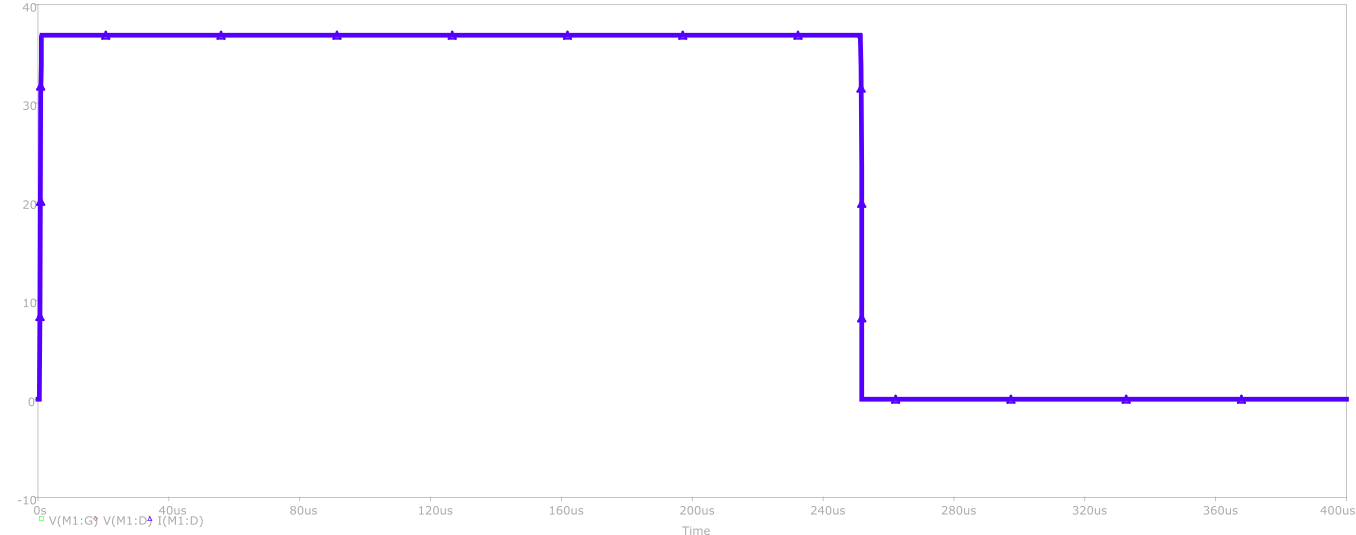
\includegraphics[width=\columnwidth]{imagenes/id_mosfet}
	\caption{Corriente de drenador $I_D$ de un MOSFET}
	\label{fig:ic_mosfet}
\end{figure}

\begin{figure}[H]
	\centering
	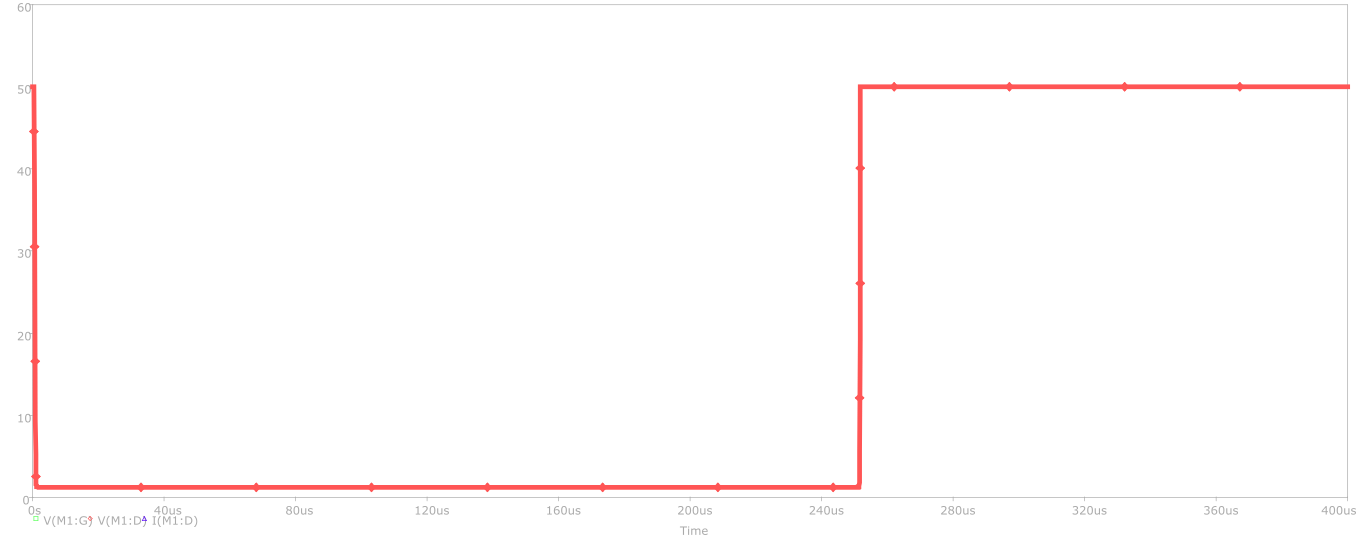
\includegraphics[width=\columnwidth]{imagenes/vds_mosfet}
	\caption{Tensión drenador-surtidor $V_{DS}$ de un MOSFET}
	\label{fig:vds_mosfet}
\end{figure}

\begin{figure}[H]
	\centering
	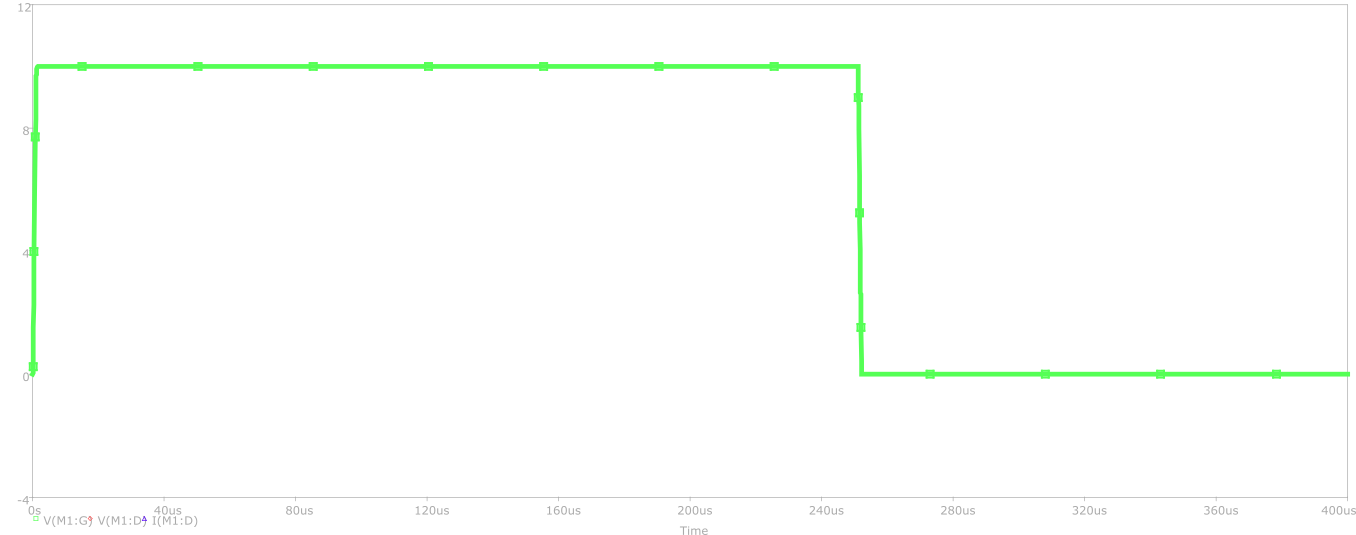
\includegraphics[width=\columnwidth]{imagenes/vgs_mosfet}
	\caption{Tensión gate-surtidor $V_{GS}$ de un MOSFET}
	\label{fig:vgs_mosfet}
\end{figure}

\begin{figure}[H]
	\centering
	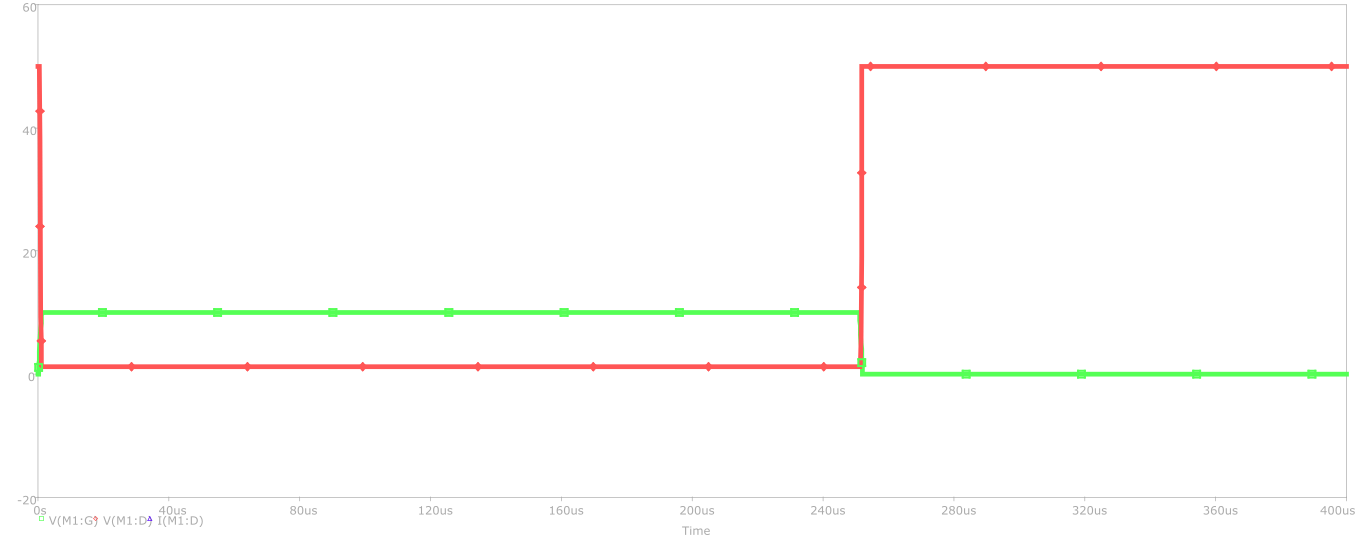
\includegraphics[width=\columnwidth]{imagenes/vds_vgs_mosfet}
\caption{$V_{DS}$ vs $V_{GS}$ de un MOSFET}
	\label{fig:vds_vgs_mosfet}
\end{figure}

Para poder cargar y descargar rápidamente las capacitancias y reducir los transitorios provocados por las inductancias, el generador de tensión del control de compuerta deberá tener una impedancia interna muy baja. La tensión máxima de compuerta no deberá excederse bajo ninguna circunstancia, debido a que esto provoca la falla del dispositivo en forma inmediata.

Puede verse en las figuras anteriores que el MOSFET posee tiempo de almacenamiento casi nulos, esto se debe a que es un dispositivo de portadores mayoritarios. 

La cantidad de $Q_{rr}$ tiene un impacto directo en el nivel de overshoot. Cuanto mayor sea el $Q_{rr}$, mayor será el overshoot. Un overshoot severo pone al dispositivo en una avalancha que puede conducir a la degradación del dispositivo con el tiempo. En otras palabras, un dispositivo con Qrr más alto es menos susceptible a un evento de conmutación difícil y duro. Por lo tanto, overshoot es un buen indicador de la robustez de la conmutación dura del dispositivo.


Cuando analizamos a los IGBT's, debemos tener en cuenta que sus características de conmutación están relacionadas con la tensión de base y con la corriente de colector. El circuito que se utiliza en este caso es el de la Fig. \ref{fig:circuit_igbt}.

\begin{figure}[H]
	\centering
	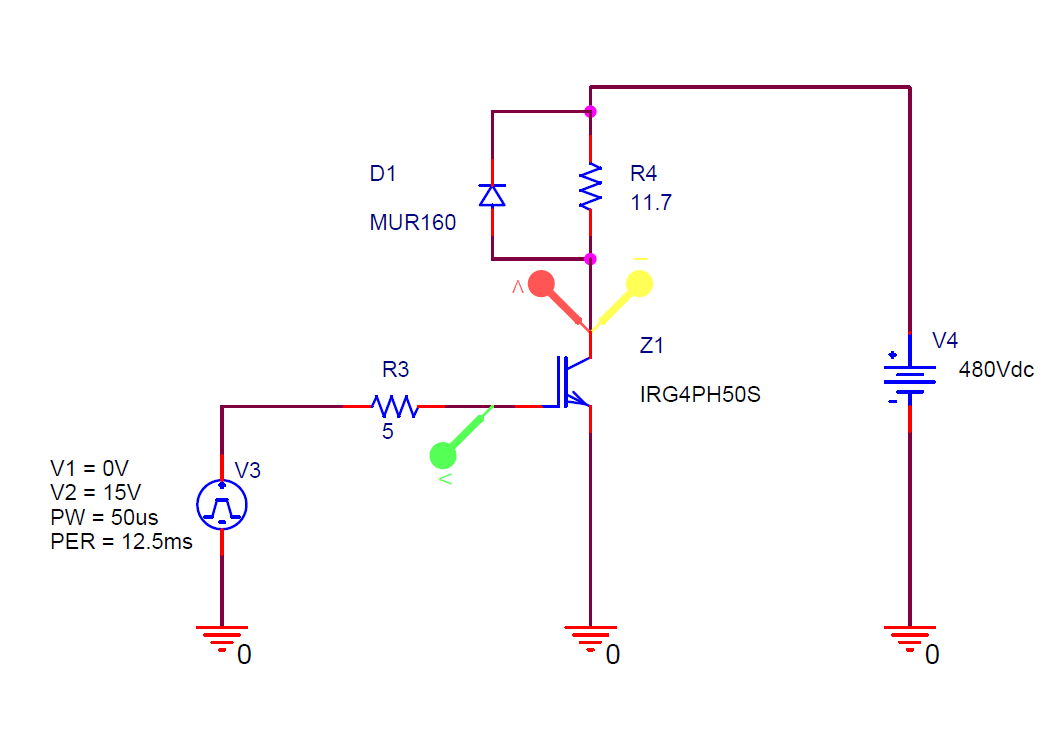
\includegraphics[width=\columnwidth]{imagenes/circuit_igbt}
	\caption{Circuito para la medición de tiempos de conmutación de un IGBT IRGPC50S}
	\label{fig:circuit_igbt}
\end{figure}

Se analizará el caso más crítico, que es cuando el transistor ya está encendido desde antes que se produzca el cortocircuito. En cuanto haya ocurrido el cortocircuito, la corriente de colector se incrementa muy vertiginosamente, esta variación de la corriente está determinada por la tensión de la conexión de continua y por la inductancia del lazo de cortocircuito.

Durante un primer momento el IGBT se encuentra desaturado, la alta variación de la tensión  colector-emisor provoca un desplazamiento de la corriente a través de la capacitancia gate-colector, la cual incrementará la tensión gate-emisor. Esto a su vez causa una corriente pico de corto circuito.
Después de tener completa la fase de desaturación, la corriente de cortocircuito cae hasta su valor estático. Durante este procedimiento, se induce un voltaje sobre la inductancia parásita, el cual aparece como un sobre pico de tensión en el IGBT. 

La fase de cortocircuito estacionario se encuentra seguida del apagado de la corriente de cortocircuito, la cual es conmutada hacia la inductancia de conmutación del circuito, la cual a su vez induce un nuevo sobre pico de tensión en el IGBT.
Estos sobre picos de tensión, inducidos durante el cortocircuito, pueden exceder los valores de operación normal durante algunos momentos. 

En las Fig. \ref{fig:ic_igbt}, \ref{fig:vge_igbt} y \ref{fig:vce_igbt}, pueden verse las gráficas de la corriente de colector, tensión gate-emisor y tensión colector-emisor, respectivamente, de un IGBT.


\begin{figure}[H]
	\centering
	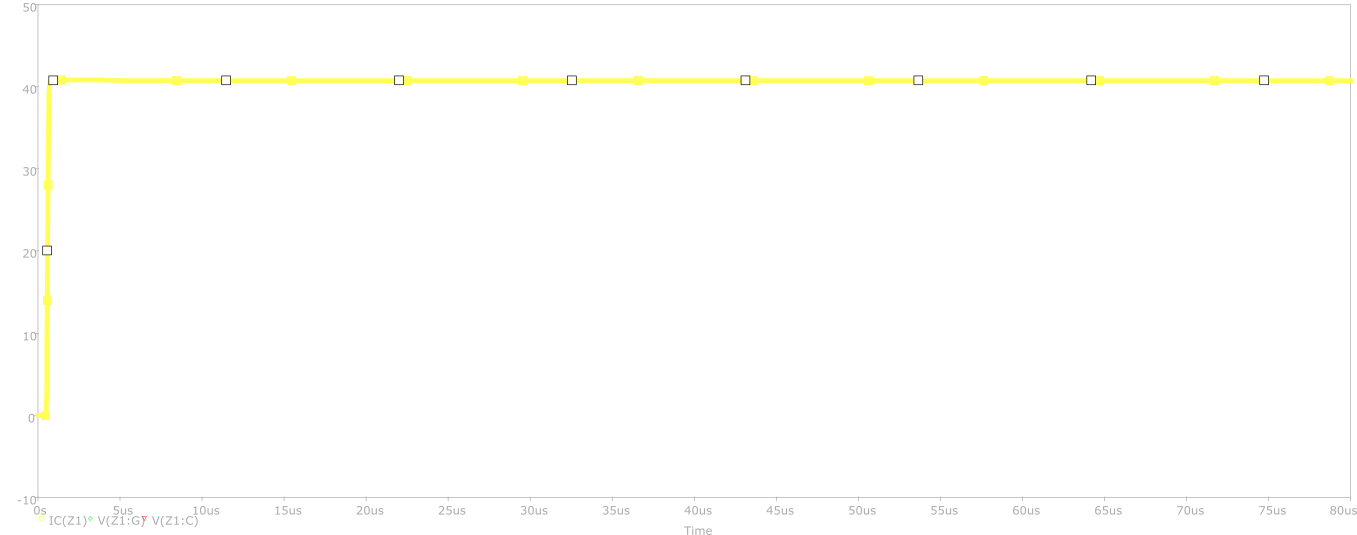
\includegraphics[width=\columnwidth]{imagenes/ic_igbt}
	\caption{Corriente de colector $I_C$ de un IGBT IRGPC50S}
	\label{fig:ic_igbt}
\end{figure}

\begin{figure}[H]
	\centering
	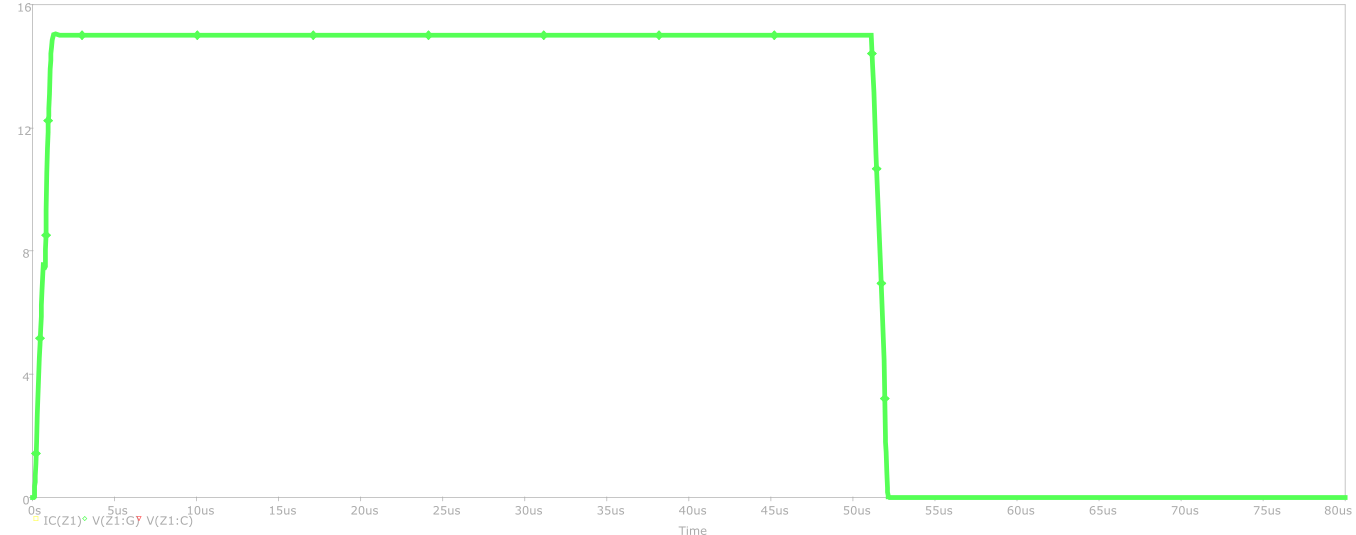
\includegraphics[width=\columnwidth]{imagenes/vge_igbt}
	\caption{Tensión gate-emisor $V_{GE}$ de un IGBT IRGPC50S}
	\label{fig:vge_igbt}
\end{figure}

\begin{figure}[H]
	\centering
	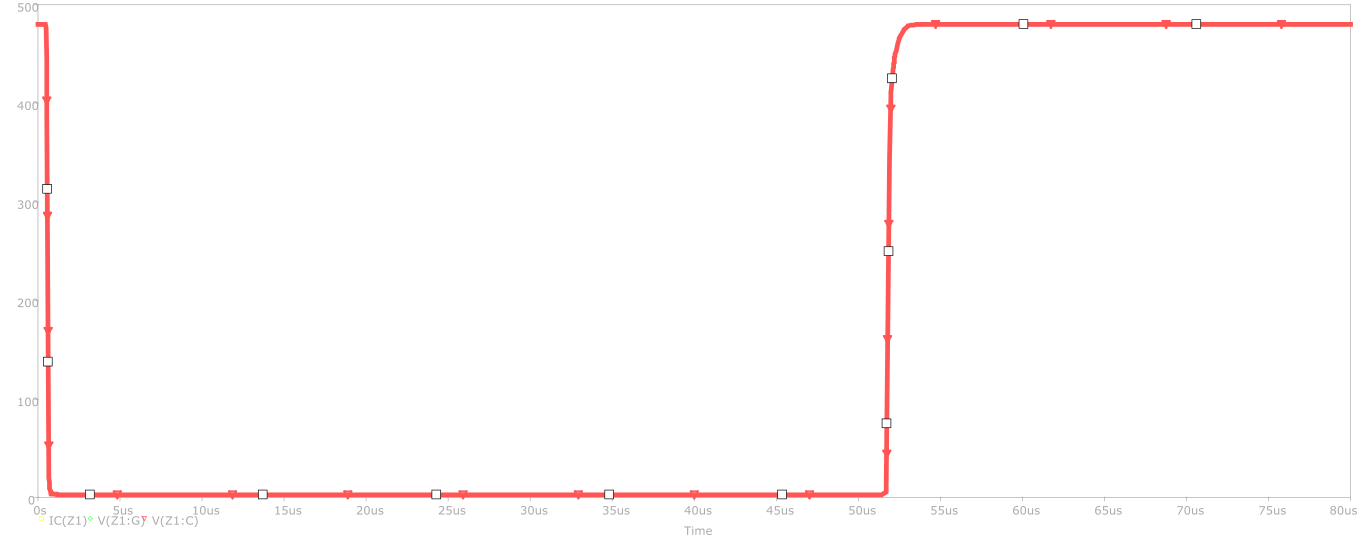
\includegraphics[width=\columnwidth]{imagenes/vce_igbt}
	\caption{Tensión colector-emisor $V_{CE}$ de un IGBT IRGPC50S}
	\label{fig:vce_igbt}
\end{figure}


Los diagramas SOA, como el de la Fig. \ref{fig:SOA}, de cortocircuito mostrados en las hojas de datos de los dispositivos muestran los limites seguros para el control de un cortocircuito.
Para garantizar una operación segura deben ser tenidos en cuenta los siguientes límites:
\begin{itemize}
	\item El tiempo entre dos cortocircuitos seguido debe se de, al menos, un segundo.
	\item El cortocircuito debe ser detectado y apagado dentro de un maximo de 10 $\mu$s.
	\item El IGBT no debe ser sometido a más de 1000 cortocircuitos durante el tiempo total de operación. 
\end{itemize}

\begin{figure}[H]
	\centering
	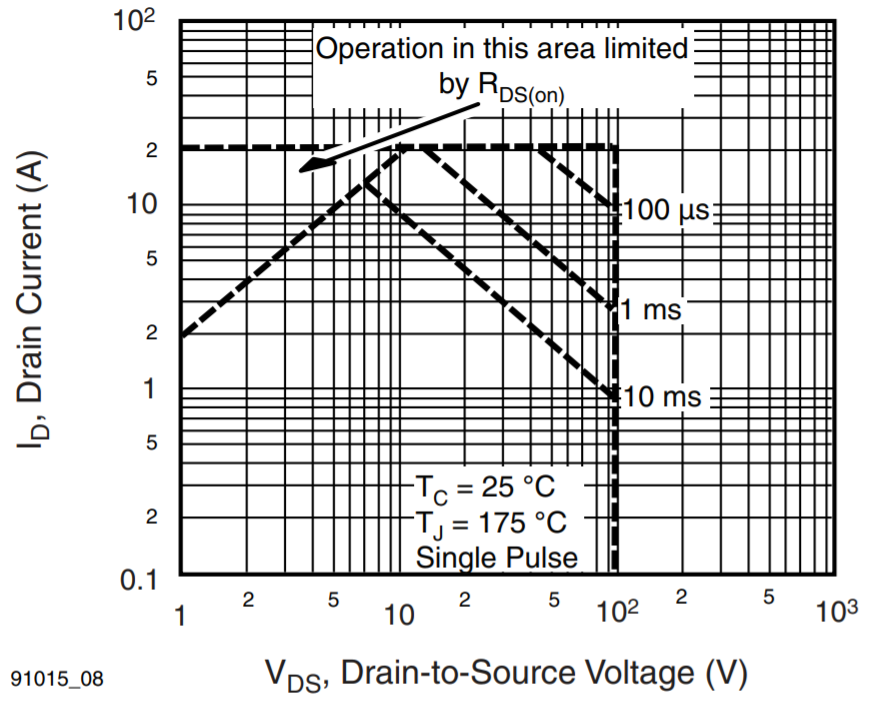
\includegraphics[width=\columnwidth]{imagenes/SOA}
	\caption{Max SOA del MOSFET IRF510}
	\label{fig:SOA}
\end{figure}

Ambos tipos de cortocircuito causan gran disipación de potencia en el transistor, lo cual incrementa la temperatura de juntura. Si el coeficiente de temperatura fuera positivo, la tensión colector emisor se vería favorecida porque habría una reducción de la corriente de colector durante el cortocircuito estacionario.
\vfill 
\section{Conclusiones}
A partir de todo lo analizado se puede comprobar que, tal como se había planteado, es posible trabajar con transistores de potencia tanto MOSFET como IGBT bajo la particular condición de cortocircuito sin que el dispositivo se vea dañado. Es válido recordar que esta condición debe ser aplicada durante períodos de tiempo muy cortos, y de ser repetitivos, el intervalo entre un cortocircuito y el otro debe ser de al menos 1s a fin de no destruir el transistor. Se pudo demostrar que el IGBT, a diferencia de MOSFET que es un dispositivo de portadores mayoritarios, tiene un tiempo de almacenamiento que limita la frecuencia de conmutación que se puede aplicar al circuito, sin embargo compensa esto con sus mejores características de conducción.\\

EL elegir dispositivos teniendo el cuenta su robustez con respecto a las condiciones de cortocircuito en aplicaciones de conmutación dura, hace que los esfuerzos de diseño puedan minimizarse al omitir los siguientes pasos de optimización o diseño:
\begin{itemize}
\item Ajuste del tiempo muerto para reducir el tiempo de conducción del diodo corporal.
\item Considerando una topología diferente para reducir la corriente de conducción del diodo.
\item Rediseño contraintuitivo de PCB para aumentar la inductancia parásita del bucle de conmutación o agregar resistencia de compuerta externa para reducir la pendiente de corriente ($\frac{d_i}{d_t}$).
\end{itemize}

De acuerdo con una variedad de proveedores, se ha decidido tomar tener en cuenta el hecho de que los métodos modernos de detección de cortocircuitos son lo suficientemente rápido como para reconocer y apagar un cortocircuito dentro de 6 $\mu$s\cite{six}. 

\vfill

\begin{thebibliography}{9}
\bibitem{IEEEhowto:kopka}
Oros, Ramón C. “Dispositivos de Potencia y convertidores de CC y CA” EDUCO. UTN. FRC. Córdoba. Argentina.Edición, Abril 2005. \\ 
`

\bibitem{IEEEhowto:kopka}
Rashid, Muhammad. “Electrónica de Potencia” Pearson Prentice Hall, México. 2015. \\


\bibitem{IEEEhowto:kopka}
Power electronics handbook : devices, circuits, and applications handbook / edited by Muhammad H. Rashid. – 3rd ed. 2011. \\


\bibitem{IEEEhowto:kopka}
Electrónica de Potencia, Daniel W. Hart; Prentice Hall, 	1995 \\

\bibitem{IEEEhowto:kopka}
Application Note Hard Diode Commutation of Power MOSFET - OptiMOS TM FD 200V/250V, March 2014\\

\bibitem{IEEEhowto:kopka}
Ensure Your System Robustness by Choosing Hard Commutation Rugged Medium Voltage MOSFETs, Alan Huang, Application Engineer, Infineon Technologies AG \\

\bibitem{six}
Application Note AN-Number: AN-2005-03 , Power electronics in motion \\

\bibitem{IEEEhowto:kopka}
Tech notes \& Data sheets On Line, Philips Semiconductors.  USA. www.Philips.com \\


\bibitem{IEEEhowto:kopka}
Tech notes \& Data sheets On Line, International RectifierInc, www.infineon.com \\

\bibitem{sc}
Short-Circuit Instabilities in Silicon IGBTs and Silicon Carbide Power MOSFETs. 2017.  Reigosa, Paula Diaz.\\

\bibitem{IEEEhowto:kopka}
Tech notes \& Data sheets On Line, Semikron Inc,
www.semikron.com \\

\bibitem{bath}
https::$//$en.wikipedia.org$/$wiki$/$Bathtub$\_$curve



\end{thebibliography}

\section{Datos biográficos}

\textbf{Facundo Emilio Navarro}, Nacido en Neuquén el 04/06/1992. Estudiante de Ingeniería en Electrónica, Universidad Tecnológica Nacional, Facultad Regional Córdoba, Argentina. Sus intereses son: Sistemas Embebidos, Procesamiento Digital de Señales, Machinne Learning.\\

e-mail: 63809@electronica.frc.utn.edu.ar 

\end{document}
